\section{Tema 5: Kronig-Penney Modellen}
\label{tema5}

\begin{table}[!htb]
    \centering
    \caption{Samtale punkter tema 4}
    \begin{tabular}{|c|c|c|r|}
      \hline
      1 & Kronig-Penney Modellen \& Forenklinger &  \autoref{sec:tema5_1} & \cellcolor{blue}\quad\quad \\
      \hline 
      2 & Bloch's teorem & \autoref{sec:tema5_3} & \cellcolor{blue} \\
      \hline
      3 & Løsningene til Kronig-Penney Modellen & \autoref{sec:tema5_4} & \cellcolor{blue} \\
      \hline 
      4 & Dispersjonsrelasjonen, E(k) & \autoref{sec:tema5_5} & \cellcolor{blue} \\
      \hline
      5 & Effektiv masse & \autoref{sec:tema5_6} & \cellcolor{blue} \\ 
      \hline
    \end{tabular}
    \label{tab:samtalePunkt_tema1}
\end{table}

\subsection{Kronig-Penney Modellen \& Forenklinger}
\label{sec:tema5_1}
Vi begynner å nærme oss gode representasjoner av atomer nå, men vi vil gjerne kunne modulere stoff. Dette gjelder også halvledere. Potensialet mellom en proton/nøytron kjerne og et elektron kan modelleres som et coulomb potensial. Dersom man ønsker å løse SL innenfor en rimelig tid, bruker man heller en forenklet modell. Denne modellen heter Kronig-Penney modellen, visualisert i figur \ref{fig:KP}

\begin{figure}[!htb]
    \centering
    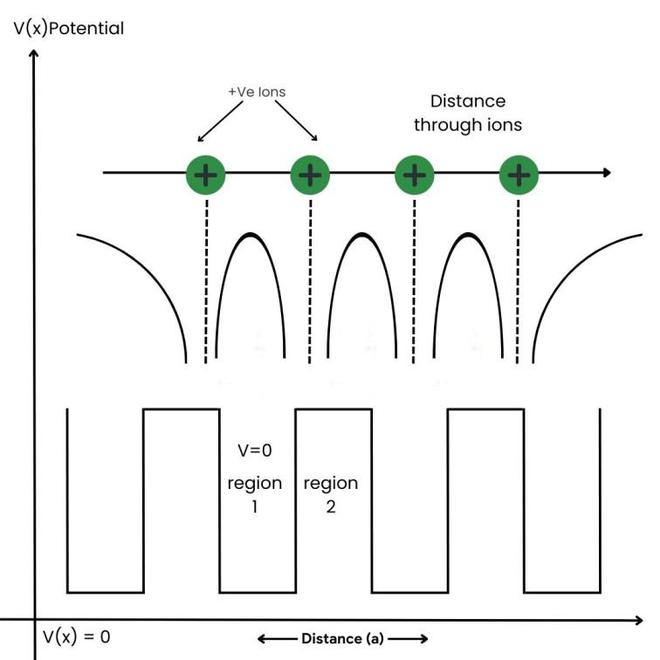
\includegraphics[scale=0.4]{Bilder/SamtaleTema5/kronigPenney.jpeg}
    \caption{Kronig-Penney modellen}
    \label{fig:KP}
\end{figure}

Ved å ta i bruk kvantebrønner kan man modellere atomer til en viss grad, energinivåene som dukker opp i brønnen tar rollen til elektronskallene. Den andre forenklingen Kronig-Penney modellen gjør er å produsere et uendelig langt gitter, dette gjør at man slipper å bry seg om rand tilfeller.

La oss se på to atomer først, dette vil virke som en dobbel kvantebrønn, slik som vi så på i \autoref{sec:tema3_7}. Om avstanden mellom de to brønnene er store, vil de i essens virke sm to uavhengige brønner. Men dersom de er nærme nok vil vi få en splitting av energinivåer (bonding nederst, og anti-bonding øvest). Splittingen blir større og større jo høyere energinivå vi har, det blir mer og mer lekkasje. 

Det er verdt å merke seg at antall energinivåer per bånd, er lik antall brønner som igjen er lik antall lineære kombinasjoner i.e. løsninger av SL. Her kommer den store nedsiden av Kronig-Penney modellen, det at det er uendelig mange brønner gjør at energien i hvert bånd er kontinuerlig, selvom det brude vært diskret.

Når vi beveger oss oppover brønnen vil det være større avstand mellom energinivåene i et bånd. Dette er fordi det er mer og mer lekkasje desto nærmere man kommer $V_0$.

\subsection{Bloch's teorem}
\label{sec:tema5_3}
Bloch's teorem sier at løsningen på SL i et periodisk potensial $V(x)$, kan uttrykket ved plane bølger modulert av en periodisk funksjon. Matematisk er det uttrykket som 

\begin{empheq}[box=\tcbhighmath]{align}
    \label{eq:bloch}
    \psi(x) = e^{ik\textbf{r}}u(\textbf{r})
\end{empheq}

Her er da $e^{ik\textbf{r}}$ planbølgen, og $u(\textbf{r})$ er en vilkårlig funksjon med samme periodisitet som krystallen. \autoref{fig:bloch} gir en visuell representasjon av ligning \ref{eq:bloch}.

\begin{figure}[!htb]
    \centering
    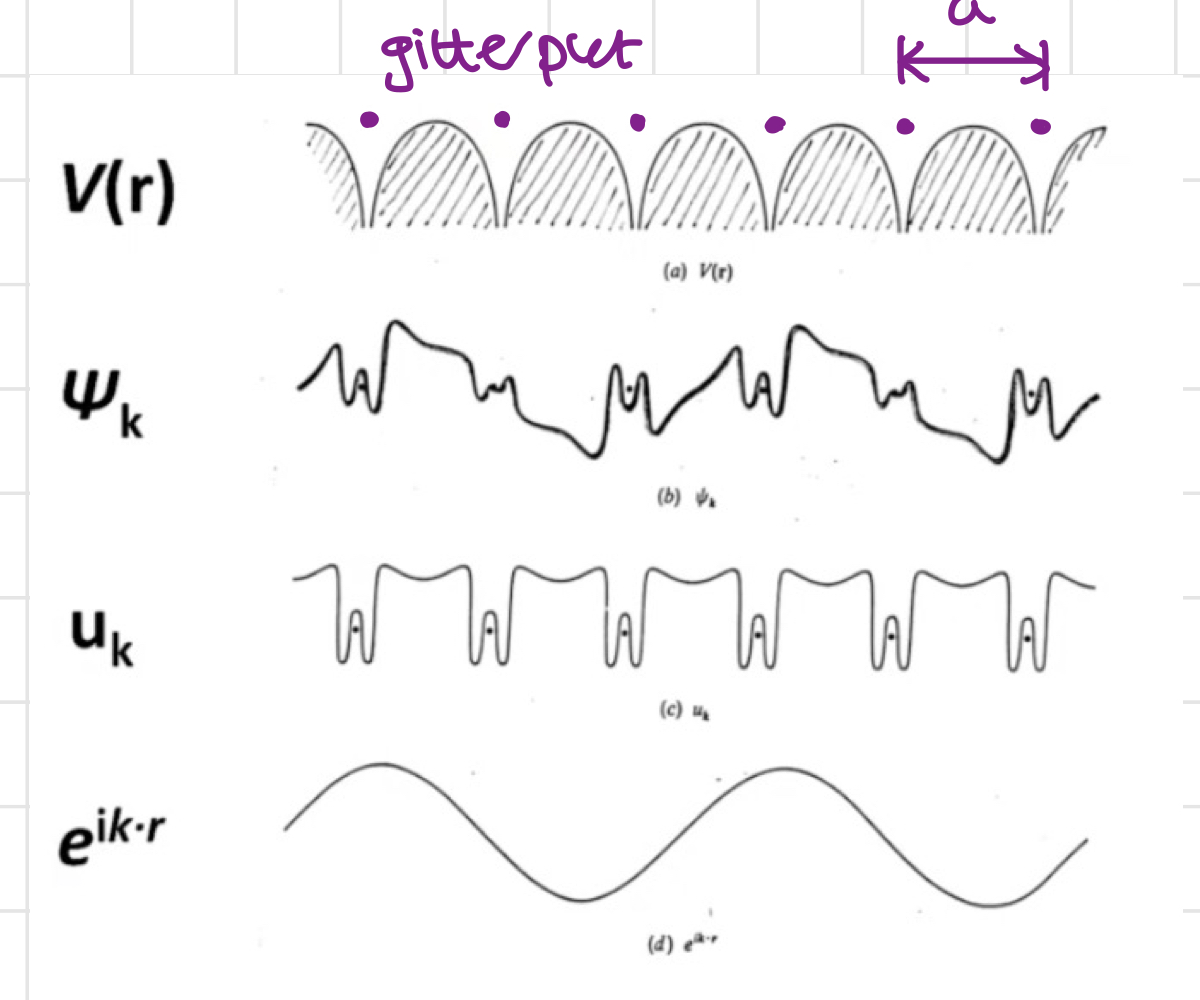
\includegraphics[scale=0.29]{Bilder/SamtaleTema5/blochs.jpeg}
    \caption{Øverst har vi potensialet til en perfekt krystall $V(\textbf{r})$. Under har vi bølgefunksjonen, denne kan dekomponeres inn i et produkt bestående av den stående bølgen nederst, og den periodiske funksjonen $u_k(\textbf{r})$ smo har samme periodisitet som $V(\textbf{r})$.}
    \label{fig:bloch}
\end{figure}

\subsection{Løsningene til Kronig-Penney Modellen}
\label{sec:tema5_4}
Utledningen av løsningen til KP-modellen er krunglette og lang og er heller ikke pensum, men resultatet av modellen er. \autoref{eq:solKP} gir en forenklet løsning av KP-modellen, men nok til å hente ut informasjonen vi trenger for å se på dispersjonsrelasjonen.

\begin{equation}
    \label{eq:solKP}
    cos(...) = sin(...)cos(..)...+cosh(...)
\end{equation}

Vi ser fra ligning \ref{eq:solKP} at vi kun kan ha løsninger mellom $-1$ og $1$. 

\begin{figure}[!htb]
    \centering
    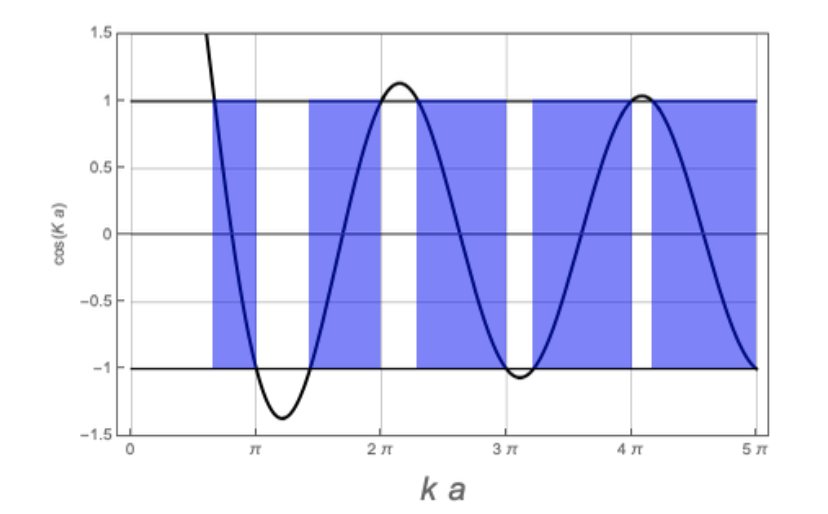
\includegraphics[scale=0.8]{Bilder/SamtaleTema5/KP-plot.png}
    \caption{Grafisk løsningen av Kronig-Penney modellen }
    \label{fig:plot-kp}
\end{figure}

$x$-aksen i dette tilfellet er en dimensjonsløs verdi som er proporsjonal med energien. Dersom vi projiserer de gyldige områdene ned på $x$-aksen og legger det oppå dispersjonslerasjonen for en fri partikkel vil vi få dispersjonsrelasjonen for Kronig-Penney modellen.

\subsection{Dispersjonsrelasjonen, E(k)}
\label{sec:tema5_5}
Som vi nevnte i slutten av \autoref{sec:tema5_4}, kan vi dersom vi legger løsningen på Kronig-Penney modellen oppå fri elektron dispersjonsrelasjonen, få ut figur \ref{fig:dispRel}

\begin{figure}[!htb]
    \centering
    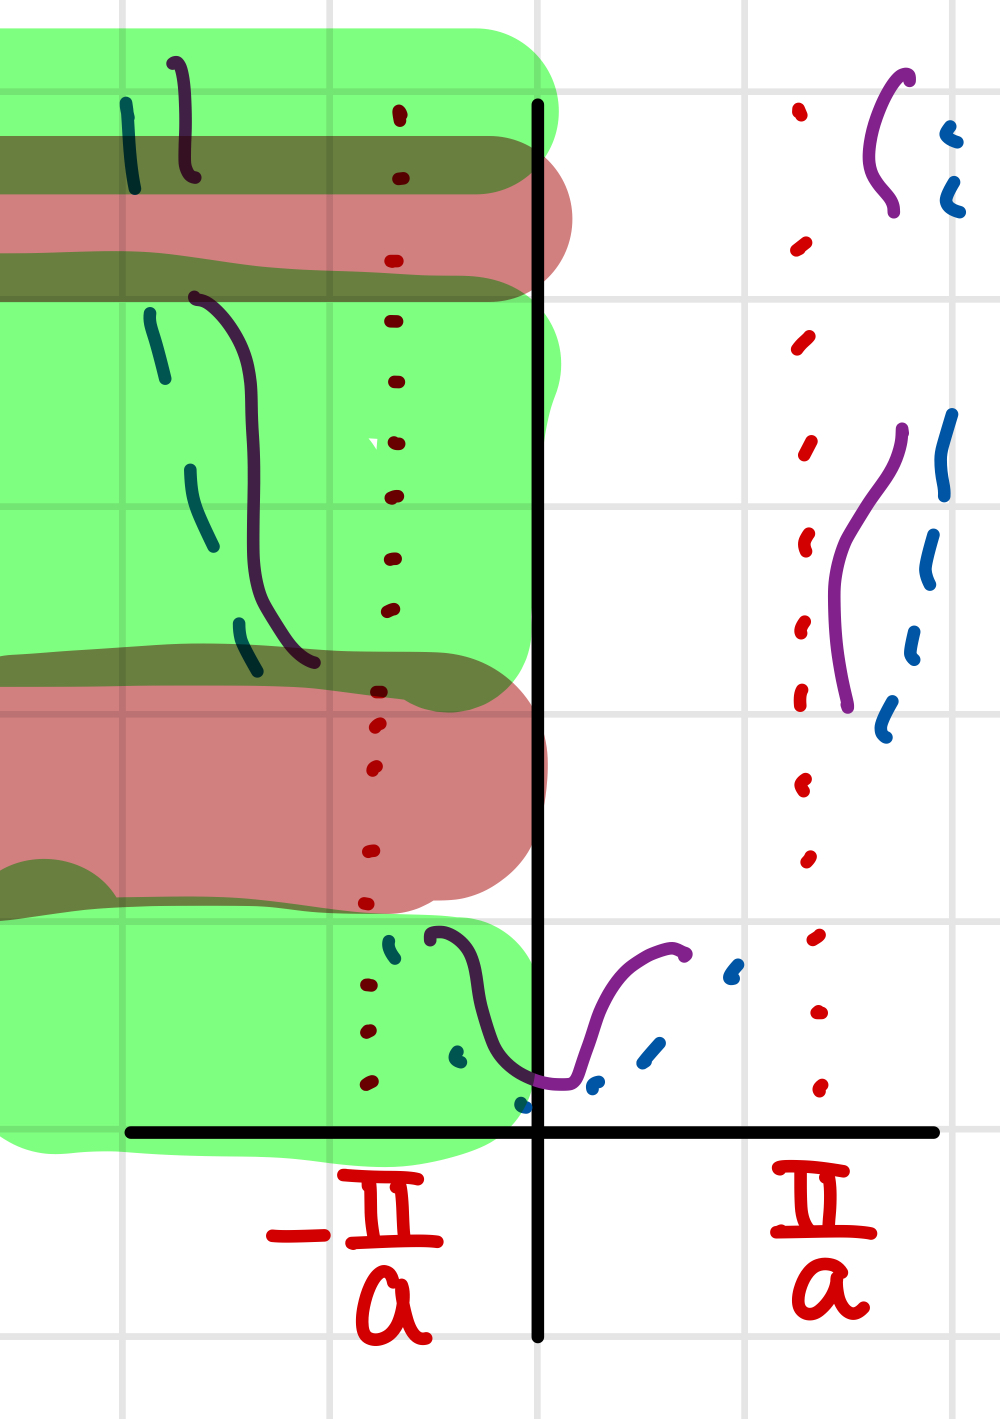
\includegraphics[scale=0.2]{Bilder/SamtaleTema5/disp-relasjon-KP.jpeg}
    \caption{Dispersjonsrelasjonen for Kronig-Penney modellen.}
    \label{fig:dispRel}
\end{figure}

Her er de grønne områdene tillate områder, disse er avhengige bølgetallet $k$ og gitterkonstanten $a$. Ved Brillouinsone grensene vil det oppstå båndgap, dette er da ved $k=\pm\frac{n\pi}{a}$.

Vi husker fra tidligere at en Brillouinsone er Wigner-Seitz cellen, men i det resiproke rom. Brillouinsonene er viktige fordi det er en representasjon av verdiene til $k$ i planbølgen som oppfyller blochs teorem.

Ved brillouinsonegrensene vil det oppstå interferens, da den reflekterte bølgen interfereres med den innkommende bølgen. Dette medfører at vi har stående bølger, og ikke kan ha energinivåer som ligger på $k = \frac{n\pi}{a}$.

Alle punkt på den lilla kurven svarer til bølgefunksjoner med bestemte k-verdier. $k$-ene er $k$-en i blochbølger ($\psi(x)=exp(ikx)u(x), \quad u(x)=u(x+a)$.

Bølger som ligger på positiv $k$-akse svarer til vandrende bølger som beveger seg i positiv $k$-retning, og det er som nevnt tidligere akkurat ved brillouinsonene at vi har betingelser som gir oss stående bølger.

$k$-en fra figur \ref{fig:dispRel} er relatert til krystallbevegelsesmengden.
\begin{equation*}
    p_{krystall} = \hbar k,
\end{equation*}

Bevegelsesmengden til det samlede systemet, dette innebærer da elektron pluss krystall. Det viser seg at $p_{krystall}$ relaterer tett til gruppehastigheten $v_g$ og er derfor et bra mål på hvordan elektron-bølgepakker beveger seg gjennom krystallen. En tilstand med postive $k$ verdier beskriver et elektron $e^-$ som beveger seg i positiv $x$-retning og andre veien for $k<0$.

Finnes flere måter å representere dispersjonsrelasjonen. \autoref{fig:reduced} viser et reduced-zone-scheme, den fra figur \ref{fig:dispRel} kalles for et extended-zone-scheme.

\begin{figure}[!htb]
    \centering
    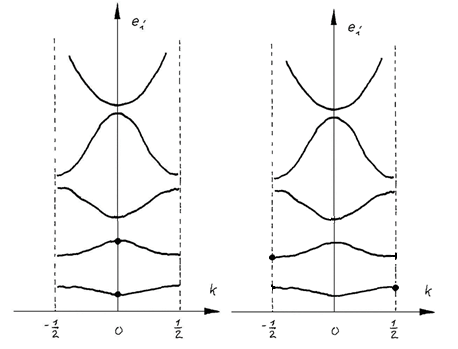
\includegraphics[scale=0.6]{Bilder/SamtaleTema5/Reduced-zone-scheme.png}
    \caption{Reduced-Zone-Scheme.}
    \label{fig:reduced}
\end{figure}

\subsection{Effektiv masse}
\label{sec:tema5_6}
Det er gunstig å kunne si noe om massen, men som vi ser fra uttrykket for energi i ligning \ref{eq:Engi} og dispersjonsrelasjonen, vil energien til en partikkel forandre seg.

\begin{equation}
\label{eq:Engi}
    E = \frac{\hbar^2k^2}{2m}
\end{equation}

Hadde vi løst ligning \ref{eq:Engi} mhp. massen, ville massen $m$ påvirkes avhengig av energien (bølgetallet $k$). Dersom vi dobbeltderiverer mhp. $k$ ser vi et forenklet uttrykk,

\begin{equation}
    \label{eq:effectiveMass}
    \begin{split}
        E &= \frac{d^2}{d k^2} \frac{\hbar^2k^2}{2m}\\
        m^* &= \frac{\hbar^2}{\frac{d^2E}{dk^2}}
    \end{split}
\end{equation}

Den effektive massen korrigerer for kreftene som virker på elektronet fra krystallen. 

Effektiv masse påvirker DOS i energi bånd, Den er med på å avgjøre hvor mange tilgjengelige tilstander det er for et gitt energinivå.

I en halvleder, så påvirker effektivmassen mobiliteten til elektronene. En lav effektiv masse gjør at elektronene er mer mobiler, og leder da strøm bedre. Kurvaturen til bånddiagrammet sier oss da noe om mobiliteten, siden den effektive massen er omvendt proporsjonal med den dobbelderiverte av energien mhp. $k$, vil en større kurvatur i  dispersjonsrelasjonen gi høyere mobilitet.